

C++11 introduced rvalue references to enable new techniques, including move semantics and perfect forwarding. This section describes the interactions between rvalue references and deduction.

\subsubsubsection{15.6.1\hspace{0.2cm}Reference Collapsing Rules}

Programmers are not allowed to directly declare a “reference to a reference”:

\begin{lstlisting}[style=styleCXX]
using RI = int&;
int i = 42;
RI r = i;
R const& rr = r; // OK: rr has type int&
\end{lstlisting}

The rules that determine the type resulting from such a composition are known as the reference collapsing rules.

\begin{tcolorbox}[colback=webgreen!5!white,colframe=webgreen!75!black]
\hspace*{0.75cm}Reference collapsing was introduced into the C++ 2003 standard when it was noted that the standard pair class template would not work with reference types. The 2011 standard extended reference collapsing further by incorporating rules for rvalue references.
\end{tcolorbox}

First, any const or volatile qualifiers applied on top of the inner reference are simply discarded (i.e., only the qualifiers under the inner reference are retained). Then the two references are reduced to a single reference according to Table 15.1, which can be summarized as “if either reference is an lvalue reference, so is the resulting type; otherwise, it is an rvalue reference.”

\begin{center}
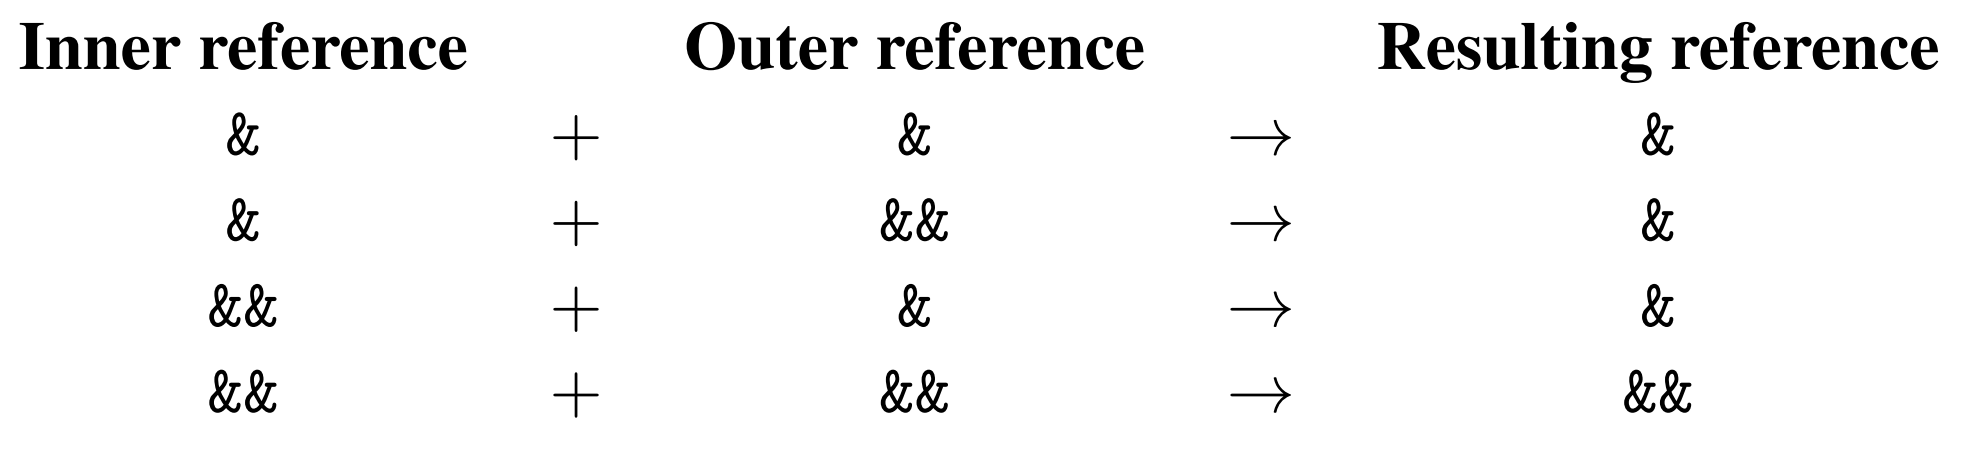
\includegraphics[width=0.8\textwidth]{content/2/chapter15/images/1.png} \\
Table 15.1. Reference Collapsing Rules
\end{center}

One more example shows these rules in action:

\begin{lstlisting}[style=styleCXX]
using RCI = int const&;
RCI volatile&& r = 42; // OK: r has type int const&
using RRI = int&&;
RRI const&& rr = 42; // OK: rr has type int&&
\end{lstlisting}


Here volatile is applied on top of the reference type RCI (an alias for int const\&) and is therefore discarded. An rvalue reference is then placed on top of that type, but since the underlying type is an lvalue reference and lvalue references “take precedence” in the reference collapsing rule, the overall type remains int const\& (or RCI, which is an equivalent alias). Similarly, the const on top of RRI is discarded, and applying an rvalue reference on top of the resulting rvalue reference type, still leaves us with an rvalue reference type in the end (which is able to bind an rvalue like 42).

\subsubsubsection{15.6.2\hspace{0.2cm}Forwarding References}

As introduced in Section 6.1 on page 91, template argument deduction behaves in a special way when a function parameter is a forwarding reference (an rvalue reference to a template parameter of that function template). In this case, template argument deduction considers not just the type of the function call argument but also whether that argument is an lvalue or an rvalue. In the cases where the argument is an lvalue, the type determined by template argument deduction is an lvalue reference to the argument type, and the reference collapsing rules (see above) ensure that the substituted parameter will be an lvalue reference. Otherwise, the type deduced for the template parameter is simply the argument type (not a reference type), and the substituted parameter is an rvalue reference to that type. For example:

\begin{lstlisting}[style=styleCXX]
template<typename T> void f(T&& p); // p is a forwarding reference

void g()
{
	int i;
	int const j = 0;
	f(i); // argument is an lvalue; deduces T to int& and
	// parameter p has type int&
	f(j); // argument is an lvalue; deduces T to int const&
	// parameter p has type int const&
	f(2); // argument is an rvalue; deduces T to int
	// parameter p has type int&&
}
\end{lstlisting}

In the call f(i) the template parameter T is deduced to int\&, since the expression i is an lvalue of type int. Substituting int\& for T into the parameter type T\&\& requires reference collapsing, and we apply the rule \& + \&\& -> \& to conclude that the resulting parameter type is int\&, which is perfectly suited to accept an lvalue of type int. In contrast, in the call f(2), the argument 2 is an rvalue and the template parameter is therefore deduced to simply be the type of that rvalue (i.e., int). No reference collapsing is needed for the resulting function parameter, which is just int\&\& (again, a parameter suited for its argument).

The deduction of T as a reference type can have some interesting effects on the instantiation of the template. For example, a local variable declared with type T will, after instantiation for an lvalue, have reference type and will therefore require an initializer:

\begin{lstlisting}[style=styleCXX]
template<typename T> void f(T&&) // p is a forwarding reference
{
	T x; // for passed lvalues, x is a reference
	...
}
\end{lstlisting}

This means that the definition of the function f() above needs to be careful how it uses the type T, or the function template itself won’t work properly with lvalue arguments. To deal with this situation, the std::remove\_reference type trait is frequently used to ensure that x is not a reference:

\begin{lstlisting}[style=styleCXX]
template<typename T> void f(T&&) // p is a forwarding reference
{
	std::remove_reference_t<T> x; // x is never a reference
	...
}
\end{lstlisting}


\subsubsubsection{15.6.3\hspace{0.2cm}Perfect Forwarding}

The combination of the special deduction rule for rvalue references and the reference collapsing rules makes it possible to write a function template with a parameter that accepts almost any argument and captures its salient properties (its type and whether it is an lvalue or an rvalue).

\begin{tcolorbox}[colback=webgreen!5!white,colframe=webgreen!75!black]
\hspace*{0.75cm}Bit fields are an exception.
\end{tcolorbox}

The function template can then “forward” the argument along to another function as follows:

\begin{lstlisting}[style=styleCXX]
class C {
	...
};

void g(C&);
void g(C const&);
void g(C&&);

template<typename T>
void forwardToG(T&& x)
{
	g(static_cast<T&&>(x)); // forward x to g()
}

void foo()
{
	C v;
	C const c;
	forwardToG(v); // eventually calls g(C&)
	forwardToG(c); // eventually calls g(C const&)
	forwardToG(C()); // eventually calls g(C&&)
	forwardToG(std::move(v)); // eventually calls g(C&&)
}
\end{lstlisting}

The technique illustrated above is called perfect forwarding, because the result of calling g() indirectly through forwardToG() will be the same as if the code called g() directly: No additional copies are made, and the same overload of g() will be selected.

The use of static\_cast within the function forwardToG() requires some additional explanation. In each instantiation of forwardToG(), the parameter x will either have lvalue reference type or rvalue reference type. Regardless, the expression x will be an lvalue of the type that the reference refers to.

\begin{tcolorbox}[colback=webgreen!5!white,colframe=webgreen!75!black]
\hspace*{0.75cm}Treating a parameter of rvalue reference type as an lvalue is intended as a safety feature, because anything with a name (like a parameter) can easily be referenced multiple times in a function. If each of those references could be implicitly treated as an rvalue, its value could be destroyed unbeknownst to the programmer. Therefore, one must explicitly state when a named entity should be treated as an rvalue. For this purpose, the C++ standard library function std::move treats any value as an rvalue (or, more precisely, an xvalue; see Appendix B for details).
\end{tcolorbox}

The static\_cast casts x to its original type and lvalue- or rvalue-ness. The type T\&\& will either collapse to an lvalue reference (if the original argument was an lvalue causing T to be an lvalue reference) or will be an rvalue reference (if the original argument was an rvalue), so the result of the static\_cast has the same type and lvalue- or rvalue-ness as the original argument, thereby achieving perfect forwarding.

As introduced in Section 6.1 on page 91, the C++ standard library provides a function template std::forward<>() in header <utility> that should be used in place of static\_cast for perfect forwarding. Using that utility template better documents the programmer’s intent than the arguably opaque static\_cast constructs shown above and prevents errors such as omitting one \&. That is, the example above is more clearly written as follows:


\begin{lstlisting}[style=styleCXX]
#include <utility>

template<typename T> void forwardToG(T&& x)
{
	g(std::forward<T>(x)); // forward x to g()
}
\end{lstlisting}

\hspace*{\fill} \\ %插入空行
\noindent
\textbf{Perfect Forwarding for Variadic Templates}

Perfect forwarding combines well with variadic templates, allowing a function template to accept any number of function call arguments and forward each of them along to another function:

\begin{lstlisting}[style=styleCXX]
template<typename... Ts> void forwardToG(Ts&&... xs)
{
	g(std::forward<Ts>(xs)...); // forward all xs to g()
}
\end{lstlisting}

The arguments in a call to forwardToG() will (independently) deduce successive values for the parameter pack Ts (see Section 15.5 on page 275), so that the types and lvalue- or rvalue-ness of each argument is captured. The pack expansion (see Section 12.4.1 on page 201) in the call to g() will then forward each of these arguments using the perfect forwarding technique explained above.

Despite its name, perfect forwarding is not, in fact, “perfect” in the sense that it does not capture all interesting properties of an expression. For example, it does not distinguish whether an lvalue is a bit-field lvalue, nor does it capture whether the expression has a specific constant value. The latter causes problems particularly when we’re dealing with the null pointer constant, which is a value of integral type that evaluates to the constant value zero. Since the constant value of an expression is not captured by perfect forwarding, overload resolution in the following example will behave differently for the direct call to g() than for the forwarded call to g():

\begin{lstlisting}[style=styleCXX]
void g(int*);
void g(...);

template<typename T> void forwardToG(T&& x)
{
	g(std::forward<T>(x)); // forward x to g()
}

void foo()
{
	g(0); // calls g(int*)
	forwardToG(0); // eventually calls g(...)
}
\end{lstlisting}

This is yet another reason to use nullptr (introduced in C++11) instead of null pointer constants:

\begin{lstlisting}[style=styleCXX]
g(nullptr); // calls g(int*)
forwardToG(nullptr); // eventually calls g(int*)
\end{lstlisting}

All of our examples of perfect forwarding have focused on forwarding the function arguments while maintaining their precise type and whether it is an lvalue or rvalue. The same problem occurs when forwarding the return value of a call to another function, with precisely the same type and value category, a generalization of lvalues and rvalues discussed in Appendix B. The decltype facility introduced in C++11 (and described in Section 15.10.2 on page 298) enables this use of a somewhat verbose idiom:

\begin{lstlisting}[style=styleCXX]
template<typename... Ts>
auto forwardToG(Ts&&... xs) -> decltype(g(std::forward<Ts>(xs)...))
{
	return g(std::forward<Ts>(xs)...); // forward all xs to g()
}
\end{lstlisting}

Note that the expression in the return statement is copied verbatim into the decltype type, so that the exact type of the return expression is computed. Moreover, the trailing return type feature is used (i.e., the auto placeholder before the function name and the -> to indicate the return type) so that the function parameter pack xs is in scope for the decltype type. This forwarding function “perfectly” forwards all arguments to g() and then “perfectly” forwards its result back to the caller.

C++14 introduced additional features to further simplify this case:

\begin{lstlisting}[style=styleCXX]
template<typename... Ts>
decltype(auto) forwardToG(Ts&&... xs)
{
	return g(std::forward<Ts>(xs)...); // forward all xs to g()
}
\end{lstlisting}

The use of decltype(auto) as a return type indicates that the compiler should deduce the return type from the definition of the function. See Section 15.10.1 on page 296 and Section 15.10.3 on page 301.

\subsubsubsection{15.6.4\hspace{0.2cm}Deduction Surprises}

The results of the special deduction rule for rvalue references are very useful for perfect forwarding. However, they can come as a surprise, because function templates typically generalize the types in the function signature without affecting what kinds of arguments (lvalue or rvalue) it allows. Consider this example:

\begin{lstlisting}[style=styleCXX]
oid int_lvalues(int&); // accepts lvalues of type int
template<typename T> void lvalues(T&); // accepts lvalues of any type
void int_rvalues(int&&); // accepts rvalues of type int
template<typename T> void anything(T&&); // SURPRISE: accepts lvalues and
// rvalues of any type
\end{lstlisting}

Programmers who are simply abstracting a concrete function like int\_rvalues to its template equivalent would likely be surprised by the fact that the function template anything accepts lvalues. Fortunately, this deduction behavior only applies when the function parameter is written specifically with the form template-parameter \&\&, is part of a function template, and the named template parameter is declared by that function template. Therefore, this deduction rule does not apply in any of the following situations:

\begin{lstlisting}[style=styleCXX]
template<typename T>
class X
{
	public:
	X(X&&); // X is not a template parameter
	X(T&&); // this constructor is not a function template
	
	template<typename Other> X(X<U>&&); // X<U> is not a template parameter
	template<typename U> X(U, T&&); // T is a template parameter from
	// an outer template
};
\end{lstlisting}

Despite the surprising behavior that this template deduction rule gives, the cases where this behavior causes problems don’t come up all that often in practice. When it occurs, one can use a combination of SFINAE (see Section 8.4 on page 129 and Section 15.7 on page 284) and type traits such as std::enable\_if (see Section 6.3 on page 98 and Section 20.3 on page 469) to restrict the template to rvalues:

\begin{lstlisting}[style=styleCXX]
template<typename T>
typename std::enable_if<!std::is_lvalue_reference<T>::value>::type
rvalues(T&&); // accepts rvalues of any type
\end{lstlisting}


























